\section{Nombre: Zopilote}   \label{per:zopilote}
\subsection{Descripción:}
Ave de rapiña, tiene un plumaje negro, su cabeza calva es de color gris oscuro y tiene un pico grisáceo.
\subsection{Status:}
Enemigo.
\subsection{Imagen}
Ver figura \ref{fig:zopilote}.
\begin{figure}
	\centering
	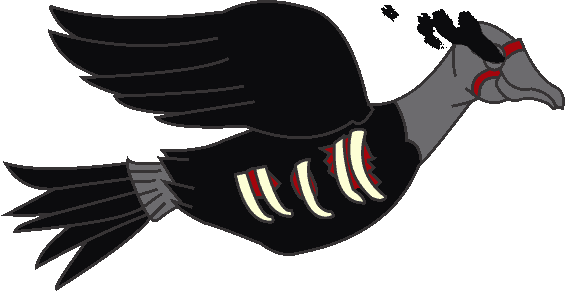
\includegraphics[height=0.2 \textheight]{Imagenes/zopilote}
	\caption{Zopilote.}
	\label{fig:zopilote}
\end{figure}
\subsection{Encuentro:}
En el nivel 5.
\subsection{Habilidades:}
\begin{itemize}
	\item Rapto. Ver habilidad en \ref{hab.rapto}.
	\item Zopilotear. Ver habilidad en \ref{hab.zopilotear}.
\end{itemize}
\subsection{Patrón de ataque:}
En un ciclo, realizará la habilidad rapto cuando se aproxime el jugador a una distancia determinada, mientras no se realice la habilidad rapto la habilidad zopilotear estará activada. Este ciclo se repetirá hasta que el enemigo desaparezca.